\documentclass{llncs}

\usepackage{ifxetex}
\ifxetex
\else
\usepackage[utf8]{inputenc}
\fi

\usepackage{amsmath}
\usepackage{mathcomp,amsfonts,amssymb,mathabx}
\usepackage[mathscr]{euscript}
\usepackage{algorithmic,algorithm}
\usepackage{paralist}
\usepackage{graphicx}
%\usepackage{color}
\usepackage{placeins}

\usepackage{enumitem}
\usepackage{dcolumn}

\usepackage{listings}
\lstset{language=C,mathescape=true,numbers=left,numbersep=0.8ex,tabsize=2,breaklines=true,basicstyle={\rm\fontfamily{phv}\small\selectfont}}

\usepackage{tikz}
\usetikzlibrary{arrows,automata,positioning}

\tikzstyle{state}=[circle,fill=black!25,minimum size=13pt,inner sep=0pt]
\tikzstyle{rstate}=[rectangle,fill=black!25,minimum size=13pt,inner sep=0pt]
\tikzstyle{transition}=[rectangle,semithick,draw=black!75,
  			  minimum size=4mm]
\tikzstyle{transition2}=[transition,rectangle,thick,dashed,
  			  minimum size=4mm]
\tikzstyle{PRstate}=[circle,double,draw,fill=blue!15,minimum size=13pt,inner sep=0pt]
\tikzstyle{polyhedra}=[blue!25,opacity=0.5,pattern=north west lines,pattern
color=blue]
\tikzstyle{line}=[black,thick]

\newcommand{\mytitle}{Succinct Representations for Abstract Interpretation}
\usepackage[pdftitle={\mytitle},pdfauthor={Julien Henry, David Monniaux, Matthieu Moy}]{hyperref}

\newcommand{\abstr}[1]{#1^\sharp}
\newcommand{\parts}[1]{\mathscr{P}(#1)}
\newcommand{\ZZ}{\mathbb{Z}}
\newcommand{\QQ}{\mathbb{Q}}
\newcommand{\RR}{\mathbb{R}}
\newcommand{\widening}{\mathop{\triangledown}}

\graphicspath{{figures/}{gnuplot/}}

% commentaires dans les algorithmes crees avec le package algorithmic
\renewcommand{\algorithmiccomment}[1]{ {\color{gray} // #1}}

\usepackage{ifthen}
\newboolean{draft}
%\setboolean{draft}{true}
\setboolean{draft}{false}

\ifthenelse{\boolean{draft}}{
  \newcommand{\avirer}[1]{{\color{red} #1}}
  \newcommand{\MM}[1]{{\color{blue} TODO(MM): #1}}
  \newcommand{\JH}[1]{{\color{teal} TODO(JH): #1}}
  \newcommand{\DM}[1]{{\color{violet} TODO(DM): #1}}
}{
  \newcommand{\avirer}[1]{}
  \newcommand{\MM}[1]{}
  \newcommand{\JH}[1]{}
  \newcommand{\DM}[1]{}
}

\title{\mytitle}
\subtitle{Combined analysis algorithms and experimental evaluation}
\author{Julien Henry\inst{1}\inst{2} \and David Monniaux\inst{1}\inst{3} \and Matthieu Moy\inst{1}\inst{4}}

\institute{VERIMAG laboratory, Grenoble, France
\and Université Joseph Fourier
\and CNRS
\and Grenoble-INP}

\renewcommand{\baselinestretch}{1}

\begin{document}
\maketitle


\begin{abstract}
Abstract interpretation techniques can be made more precise by distinguishing
paths inside loops, at the expense of possibly exponential complexity. SMT-solving techniques and sparse representations of paths and sets of paths avoid this pitfall.

We improve previously proposed techniques for guided static analysis and the generation of disjunctive invariants by combining them with techniques for succinct representations of paths and symbolic representations for transitions based on static single assignment.

Because of the non-monotonicity of the results of abstract interpretation with widening operators, it is difficult to conclude that some abstraction is more precise than another based on theoretical local precision results. We thus conducted extensive comparisons between our new techniques and previous ones, on a variety of open-source packages.
\end{abstract}


\section{Introduction}
Static analysis by abstract interpretation is a fully automatic program analysis method. When applied to imperative programs, it computes an inductive invariant mapping each program location (or a subset thereof) to a set of states represented symbolically~\cite{CousotCousot_JLC92}.
For instance, if we are only interested in scalar numerical program variables, such a set may be a convex polyhedron (the set of solutions of a system of linear inequalities)~\cite{CousotHalbwachs78,Halbwachs_PhD,PPL,BagnaraHZ08SCP}.

In such an analysis, information may flow forward \avirer{(one computes the polyhedron after a program statement as the image by the semantics of the statement, or a super-set thereof, of the polyhedron before)} or backward;
forward program analysis computes super-sets of the states reachable from the initialization of the program, backward program analysis computes super-sets of the states co-reachable from some property of interest (for instance, the violation of an assertion).
In forward analysis, control-flow joins correspond to convex hulls if using convex polyhedra (more generally, they correspond to least upper bounds in a lattice); in backward analysis, it is control-flow splits that correspond to convex hulls.

It is a known limitation of program analysis by abstract interpretation that this convex hull, or more generally, least upper bound operation, may introduce states that cannot occur in the real program: for instance, the convex hull of the intervals $[-2,-1]$ and $[1,2]$ is $[-2,2]$, strictly larger than the union of the two.
Such introduction may prevent proving desired program properties, for instance $\neq 0$. The alternative is to keep the union symbolic (e.g. compute using $[-2,-1] \cup [1,2]$) and thus compute in the \emph{disjunctive completion}
of the lattice, but the number of terms in the union may grow exponentially with the number of successive tests in the program to analyze, not to mention difficulties for designing suitable widening operators for enforcing the convergence of fixpoint iterations~\cite{PPL,BagnaraHZ08SCP,DBLP:journals/sttt/BagnaraHZ07}.
The exponential growth of the number of terms in the union may be controlled by heuristics that judiciously apply least upper bound operations, as in the \emph{trace partitioning domain} \cite{Rival_Mauborgne_TOPLAS07} implemented in the Astr\'ee analyzer~\cite{ASTREE_PLDI03,ASTREE_ESOP05}.

Assuming we are  interested in a loop-free program fragment, the above approach of keeping symbolic unions gives the same results as performing the analysis separately over every path in the fragment.
A recent method for finding disjunctive loop invariants \cite{DBLP:conf/pldi/GulwaniZ10} is based on this idea: each path inside the loop body is considered separately.
Two recent proposals use SMT-solving \cite{Kroening_Strichman_08} as a decision procedure for the satisfiability of first-order arithmetic formulas in order to enumerate only paths that are needed for the progress of the analysis \cite{Gawlitza_Monniaux_ESOP11,Monniaux_Gonnord_SAS11}. They can equivalently be seen as analyses over a multigraph of transitions between some distinguished control nodes. This multigraph has an exponential number of edges, but is never explicitly represented in memory; instead, this graph is \emph{implicitly} or \emph{succinctly} represented: its edges are enumerated as needed as solutions to SMT problems.

An additional claim of the methods that distinguish paths inside the loop body \cite{DBLP:conf/pldi/GulwaniZ10,Monniaux_Gonnord_SAS11} is that they tend to generate better invariants than methods that do not, by behaving better with respect to the \emph{widening operators} \cite{CousotCousot_JLC92}
used for enforcing convergence when searching for loop invariants by Kleene iterations. A related technique, \emph{guided static analysis} \cite{DBLP:conf/sas/GopanR07}, computes successive loop invariants for increasing subsets of the transitions taken into account, until all transitions are considered; again, the claim is that this approach avoids some gross over-approximation introduced by widenings.

All these methods improve the precision of the analysis by keeping the
same abstract domain (say, convex polyhedra) but changing the
operations applied and their ordering. An alternative is to change the
abstract domain (e.g. octagons, convex polyhedra
\cite{DBLP:journals/lisp/Mine06}), or the widening
operator~\cite{BagnaraHRZ05SCP,Polka:FMSD:97}.

\avirer{There are many possible combinations of the above techniques, and it is not
evident which ones perform more or less precisely or more or less efficiently on real-life examples. One needs to experiment.
Unfortunately, the published literature on the subject lacks experimental comparative assessments. One purpose of this article is therefore to propose such experimental results.}

This article makes the following contributions:
\begin{compactenum}
\item We recast the guided static analysis technique from \cite{DBLP:conf/sas/GopanR07} on the expanded multigraph from \cite{Monniaux_Gonnord_SAS11}, considering entire paths instead of individual transitions, using SMT queries and binary decision diagrams\label{contr:guided_multigraph} (See \S\ref{sec:guided_multigraph}).
\item We improve the technique for obtaining disjunctive invariants from \cite{DBLP:conf/pldi/GulwaniZ10} by replacing the explicit exhaustive enumeration of paths by a sequence of SMT queries\label{contr:disjunctive} (See \S\ref{sec:disjunctive}).
\item We implemented these techniques, in addition to ``classical'' iterations and the original guided static analysis, inside a prototype static analyzer.
This tool uses the LLVM bitcode format \cite{Lattner:2004:LCF:977395.977673,LLVM_langref} as input, which can be produced by compilation from C, C++ and Fortran, enabling it to be run on many real-life programs.
It uses the APRON library \cite{DBLP:conf/cav/JeannetM09}, which
supports a variety of abstract domains for numerical variables, from
which we can choose with minimal changes to our analyzer.

\avirer{
Our tool uses a \emph{single static assignment} (SSA) intermediate representation, which allows us to perform cheap symbolic propagations and simplifications,
described in Section~\ref{sec:analysis-algorithm}.
}

\item We conducted extensive experiments with this tool, on real-life programs\avirer{: (i) fixing the abstract domain, varying the iteration technique (\S\ref{sec:compare_techniques}) (ii) fixing the iteration technique, varying the abstract domain (\S\ref{sec:compare_domains})}.
\end{compactenum}

\section{Bases}
\subsection{Static Analysis by Abstract Interpretation}
\label{sec:static_analysis}
\MM{On peut peut-être réduire un peu vu que tout le monde connait à
  SAS ?}

Let $X$ be the set of possible states of the program variables; for instance, if the program has 3 unbounded integer variables, then $X = \ZZ^3$. The set $\parts{X}$ of subsets of $X$, partially ordered by inclusion, is the \emph{concrete domain}. An \emph{abstract domain} is a set $\abstr{X}$ equipped with a partial order $\sqsubseteq$; for instance, it can be the domain of convex polyhedra in $\QQ^3$ ordered by geometric inclusion. \avirer{In this article, all abstract domains are supposed to contain machine-representable objects, and all $\sqsubseteq$ order relations are supposed to be decidable.}
The concrete and abstract domains are connected by a monotone \emph{concretization} function $\gamma: \left(\abstr{X},\sqsubseteq\right) \rightarrow (\parts{X},\subseteq)$: an element $\abstr{x} \in \abstr{X}$ represents a set $\gamma(\abstr{x})$.%
%
% \footnote{%
% Some presentations of abstract interpretation identify an element $\abstr{x}$ with the set of states $\gamma(\abstr{x})$ that it represents. This leads to simpler notations, but may also confuse if, as in some of our constructions, there exist several $\abstr{x}$ with identical $\gamma(\abstr{x})$, but distinct algorithmic behaviors.}

We also assume a join operator $\sqcup: \abstr{X} \times \abstr{X} \rightarrow \abstr{X}$, with infix notation; in practice, it is generally a least upper bound operation, but we only need it to satisfy $\gamma(\abstr{x}) \cup \gamma(\abstr{y}) \subseteq \gamma(\abstr{x} \sqcup \abstr{y})$ for all $\abstr{x},\abstr{y}$.

Classically, one considers the control-flow graph of the program, with edges labeled with concrete transition relations (e.g. $x' = x+1$ for an instruction \lstinline|x = x+1;|), and attaches an abstract element to each control point.
A concrete transition relation $\tau \subseteq X \times X$ is replaced by an abstract \emph{forward abstract transformer} $\abstr{\tau}: \abstr{X} \rightarrow \abstr{X}$, such that
\(
\forall \abstr{x} \in \abstr{X}, x,x' \in X,~
x \in \gamma(\abstr{x}) \land (x,x') \in \tau \implies
x' \in \gamma \circ \abstr{\tau}(\abstr{x})
\).
It is easy to see that if to any control point $p \in P$ we attach an abstract element $\abstr{x}_p$ such that
(i) for any $p$, $\gamma(\abstr{x}_p)$ includes all initial states possible at control node $p$
(ii) for any $p,p'$, $\abstr{\tau}_{p,p'} (\abstr{x}_p) \sqsubseteq \abstr{x}_{p'}$, noting $\tau_{p,p'}$ the transition from $p$ to~$p'$, then $(\gamma(\abstr{x}_p))_{p \in P}$ form an \emph{inductive invariant}: by induction, when the control point is $p$, the program state always lies in $\gamma(\abstr{x}_p)$.

\emph{Kleene iterations} compute such an inductive invariant as the stationary limit, if it exists, of the following system: for each $p$, initialize $\abstr{x}_p$ such that $\gamma(\abstr{x}_p)$ is a superset of the initial states at point $p$; then iterate the following:
if $\abstr{\tau}_{p,p'} (\abstr{x}_p) \nsqsubseteq \abstr{x}_{p'}$, replace $\abstr{x}_{p'}$ by $\abstr{x}_{p'} \sqcup \abstr{\tau}_{p,p'} (\abstr{x}_p)$.
Such a stationary limit is bound to exist if $\abstr{X}$ has no infinite ascending chain $a_1 \sqsubsetneq a_2 \sqsubsetneq \dots$; this condition is however not met by domains such as intervals or convex polyhedra.

\emph{Widening-accelerated Kleene iterations} proceed by replacing $\abstr{x}_{p'} \sqcup \abstr{\tau}_{p,p'} (\abstr{x}_p)$ by $\abstr{x}_{p'} \widening (\abstr{x}_{p'} \sqcup \abstr{\tau}_{p,p'} (\abstr{x}_p))$ where $\widening$ is a \emph{widening operator}: for all $\abstr{x},\abstr{y}$, $\gamma(\abstr{y}) \subseteq \gamma(\abstr{x} \widening \abstr{y})$, and there exists no sequence $\abstr{u}_1,\abstr{u}_2,\dots$ of the form $\abstr{u}_{n+1} = \abstr{u}_n \widening \abstr{v}_n$ where $\abstr{v}_n$ is another sequence.
Such iterations necessarily lead to a stationary limit $(\abstr{x}_p)_{p \in P}$, which defines an inductive invariant $(\gamma(\abstr{x}_p))_{p \in P}$. Note that this invariant is not, in general, the least one expressible in the abstract domain, and may depend on the iteration ordering (the successive choices~$p,p'$).

Once an inductive invariant $\gamma((\abstr{x}_p)_{p \in P})$ has been obtained,
one can attempt \emph{decreasing} or \emph{narrowing} iterations to reduce it.
In their simplest form, this just means running the following operation until a
fixpoint or a maximal number of iterations are reached: for any $p'$, replace
$\abstr{x}_{p'}$ by $\abstr{x}_{p'} \cap \left(\bigsqcup_{p \in P}
\abstr{\tau}_{p,p'} (\abstr{x}_p)\right)$. The result also defines an inductive
invariant. These decreasing iterations are indispensable to recover properties
from guards (tests) in the program in most iteration settings; unfortunately,
certain loops, particularly those involving identity (no-operation) transitions,
may foil them: the iterations immediately reach a fixpoint and do not decrease
further (see example in \S\ref{subsec:rate_lim}). Sections \ref{sec:guided} and
\ref{sec:path_focusing} describe techniques that work around this problem.

\MM{J'avais insisté pour qu'on écrive un truc comme ça, mais si on ne
  met plus l'accent sur le côté expérimental, on peut sans doute
  supprimer ce paragraphe completement ?}
\avirer{
Widening operations have a somewhat counterintuitive behavior: the
result of an analysis (postcondition) is not necessarily monotonic
with respect to the precondition.
% For instance, classical interval
% analysis with widening and decreasing iterations on the loop
% \lstinline|while (x != 10) x=x+1;| yields a loop invariant $x \in
% [0,+\infty)$ if the precondition is $x \in [0,0]$, but $x \in [0,10]$
% (strictly stronger) if the precondition is $x \in [0,10]$ (strictly
% weaker).
This means that, when using widenings, being locally more precise \avirer{(for instance, by using more expressive abstract domains, or widening operators that climb more slowly \cite{BagnaraHRZ05SCP})} does not necessarily translate into higher final precision.
% It is almost always possible to concoct examples where a supposedly more precise abstraction (e.g. polyhedra) yields less precise results than a less precise one (e.g. intervals), but are these examples representative of real programs
This justifies our recourse to evaluation on real, large programs~(\S~\ref{sec:compare_techniques}).
}

\subsection{SMT-solving}
Boolean satisfiability (SAT) is the canonical NP-complete problem: given a propositional formula (e.g. $(a \lor \neg b) \land (\neg a \lor b \lor \neg c)$), decide whether it is satisfiable --- and, if so, output a satisfying assignment.
Despite an exponential worst-case complexity, the DPLL algorithm \cite{Kroening_Strichman_08,Handbook_SAT} solves many useful SAT problems in practice.

SAT was extended to \emph{satisfiability modulo theory} (SMT): in addition to propositional literals, SMT formulas admit atoms from a theory.
For instance, the theories of linear integer arithmetic (LIA) and linear real arithmetic (LRA) have atoms of the form $a_1 x_1 + \dots + a_n x_n \bowtie C$ where $a_1,\dots,a_n,C$ are integer constants, $x_1,\dots,x_n$ are variables (interpreted over $\ZZ$ for LIA and $\RR$ or $\QQ$ for LRA), and $\bowtie$ is a comparison operator $=,\neq,<,\leq,>,\geq$.
Satisfiability for LIA and LRA is NP-complete, yet tools based on DPLL(T) approach \cite{Kroening_Strichman_08,Handbook_SAT} solve many useful SMT problems in practice. All these tools provide a \emph{satisfying assignment} if the problem is satisfiable.

\avirer{
Most SMT solvers, including Z3,
%\footnote{\url{http://research.microsoft.com/en-us/um/redmond/projects/z3/}}
Yices,
%\footnote{\url{http://yices.csl.sri.com/}}
and all those supporting the full SMTLIB2 standard \cite{BarST-SMTLIB},
offer an \emph{incremental} interface: the client program specifies the formula as an initially empty conjunction, to which additional constraints are added, and calls a ``check'' function answering whether it is satisfiable; 
it may then backtrack some of the constraints and add other ones without restarting from scratch.
}

\subsection{A Simple, Motivating Example}
\label{subsec:rate_lim}
Consider the following program, adapted from \cite{Monniaux_Gonnord_SAS11}, where \lstinline|input($a$, $b$)| stands for a nondeterministic input in $[a,b]$:
\lstinputlisting{rlim_int.c}
This program implements a construct commonly found in control programs (in e.g.
automotive or avionics): a rate limiter.
\avirer{For the sake of simplicity, we chose it
to be fed on a nondeterministic input clamped between $[-100000,100000]$, but in a real system it would be integrated in a reactive control loop and its input connected to a complex system with unknown output range.}

The expected inductive invariant is $\lstinline|x_old| \in [-100000,100000]$, but classical abstract interpretation using intervals (or octagons or polyhedra) finds $\lstinline|x_old| \in (-\infty,+\infty)$~\cite{ASTREE_ESOP05}.
Let us briefly see why.

Widening iterations converge to $\lstinline|x_old| \in (-\infty,+\infty)$; let us now see why decreasing iterations fail to recover the desired invariant.
The \lstinline|x > x_old+10| test at line~6, if taken, yields $\lstinline|x_old|
\in (-\infty,99990)$; followed by \lstinline|x = x_old+10|, we obtain
$\lstinline|x| \in (-\infty,\allowbreak 100000)$, and the same after union with the no-operation ``else'' branch. Line~7 yields $\lstinline|x| \in (-\infty,+\infty)$.

We could use ``widening up to'' or ``widening with thresholds'', propagating the ``magic values'' $\pm 100000$ associated to \lstinline|x| into \mbox{\lstinline|x_old|,} but these syntactic approaches cannot directly cope with programs for which $\lstinline|x|  \in [-100000,+100000]$ is itself obtained by analysis.
The guided static analysis of \cite{DBLP:conf/sas/GopanR07} does not perform
better, and also obtains $\lstinline|x_old| \in (-\infty,+\infty)$.

In contrast, let us distinguish all four possible execution paths through the tests at lines 6 and~7. The path through both ``else'' branches is infeasible; the program is thus equivalent to:
\lstinputlisting{rlim_int2.c}

\avirer{
\begin{figure}
\MM{J'aime bien cette figure, qui montre en un coup d'oeil l'idée,
  mais elle prend vraiment beaucoup de place, je propose de
  supprimer.}

\centering
\begin{minipage}[c]{.21\textwidth}
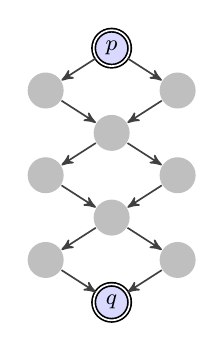
\begin{tikzpicture}[->,>=stealth',auto,node distance=.2cm and .5cm,
                    semithick,font=\footnotesize]

	\node[PRstate] (n0) {$p$};
	\node[state] (n1) [below left=of n0] {};
	\node[state] (n2) [below right=of n0] {};
	\node[state] (n3) [below right=of n1] {};
	\node[state] (n4) [below left=of n3] {};
	\node[state] (n5) [below right=of n3] {};
	\node[state] (n6) [below right=of n4] {};
	\node[state] (n7) [below left=of n6] {};
	\node[state] (n8) [below right=of n6] {};
	\node[PRstate] (n9) [below right=of n7] {$q$};

  \path [transition] (n0) -- (n1);
  \path [transition] (n0) -- (n2);
  \path [transition] (n1) -- (n3);
  \path [transition] (n2) -- (n3);
  \path [transition] (n3) -- (n4);
  \path [transition] (n3) -- (n5);
  \path [transition] (n4) -- (n6);
  \path [transition] (n5) -- (n6);
  \path [transition] (n6) -- (n7);
  \path [transition] (n6) -- (n8);
  \path [transition] (n7) -- (n9);
  \path [transition] (n8) -- (n9);
\end{tikzpicture}
\end{minipage} 
$\Longrightarrow$
\begin{minipage}[c]{.19\textwidth}
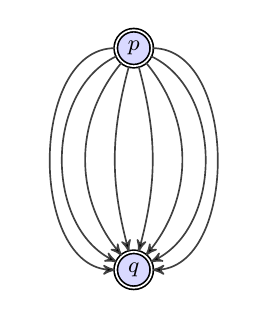
\begin{tikzpicture}[->,>=stealth',auto,node distance=.2cm and .5cm,
                    semithick,font=\footnotesize]

	\node[PRstate] (n0) {$p$};
	\node (n1) [below left=of n0] {};
	\node (n2) [below right=of n0] {};
	\node (n3) [below right=of n1] {};
	\node (n4) [below left=of n3] {};
	\node (n5) [below right=of n3] {};
	\node (n6) [below right=of n4] {};
	\node (n7) [below left=of n6] {};
	\node (n8) [below right=of n6] {};
	\node[PRstate] (n9) [below right=of n7] {$q$};

  \path [transition] 
		(n0) edge  [out=0, in=0]            node {} (n9);
  \path [transition] 
		(n0) edge  [out=180, in=180]        node {} (n9);
  \path [transition] 
		(n0) edge  [out=205, in=155]            node {} (n9);
  \path [transition] 
		(n0) edge  [out=230, in=130]            node {} (n9);
  \path [transition] 
		(n0) edge  [out=255, in=105]            node {} (n9);
  \path [transition] 
		(n0) edge  [out=-25, in=25]            node {} (n9);
  \path [transition] 
		(n0) edge  [out=-50, in=50]            node {} (n9);
  \path [transition] 
		(n0) edge  [out=-75, in=75]            node {} (n9);
\end{tikzpicture}
\end{minipage}
\caption{Expansion of the transition graph into a multigraph.}
\label{fig:multigraph}
\end{figure}
}

Classical interval analysis on this program yields $\lstinline|x_old| \in [-100000,100000]$.
We have transformed the program, manually pruning out infeasible paths; yet in general the resulting program could be exponentially larger than the first \avirer{(as in Fig.~\ref{fig:multigraph})}, even though not all feasible paths are needed to compute the invariant.

Following recent suggestions \cite{Gawlitza_Monniaux_ESOP11,Monniaux_Gonnord_SAS11}, we avoid this space explosion by keeping the second program implicit while simulating its analysis. This means we work on an implicitly represented transition multigraph \avirer{(Fig.~\ref{fig:multigraph})}; it is succinctly representated by the transition graph of the first program.
Our first contribution (\S\ref{sec:guided_multigraph}) is to recast the ``guided analysis'' from \cite{DBLP:conf/sas/GopanR07} on such a succinct representation of the paths in lieu of the individual transitions.
A similar explosion occurs in disjunctive invariant generation, following \cite{DBLP:conf/pldi/GulwaniZ10}; our second contribution (\S\ref{sec:disjunctive}) applies our implicit representation to their method.


\subsection{Guided Static Analysis}
\label{sec:guided}
\emph{Guided static analysis} was proposed by \cite{DBLP:conf/sas/GopanR07} as an improvement over classical upward Kleene iterations with widening.
Consider the program in Fig.~\ref{fig:gopan_reps_invariant}, taken from \cite{DBLP:conf/sas/GopanR07}.

\begin{figure}
  \vspace{-1em}
  \begin{minipage}{.3\linewidth}
    \lstinputlisting[label=lst:gopan_reps]{gopan_reps.c}
  \end{minipage}
\hfill
\begin{minipage}{.5\linewidth}
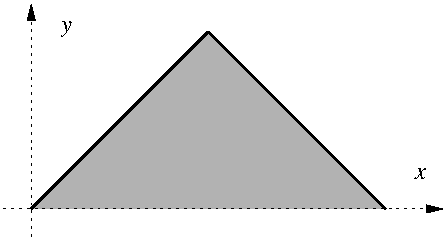
\includegraphics[scale=0.7]{gopan_reps}
\vspace{-1em}
\begin{equation}
y \leq x \;\land\; y \leq 102-x \;\land\; y \geq 0.\label{eqn:triangle}
\end{equation}
\end{minipage}
\caption{Example program and its invariant: the piecewise linear, solid line is the strongest invariant, the grayed polyhedron is its convex hull.}
\label{fig:gopan_reps_invariant} 
\end{figure}

Classical iterations on the domain of convex polyhedra \cite{CousotHalbwachs78,BagnaraHRZ05SCP} or octagons \cite{DBLP:journals/lisp/Mine06} start with $x = 0 \land x = 0$, then continue with $x = y \land 0 \leq x \leq 1$.
The widening operator extrapolates from these two iterations and yields $x = y \land x \geq 0$.
From there, the ``else'' branch at line 5 may be taken; with further widening, $0 \leq y \leq x$ is obtained as a loop invariant, and thus the postcondition computed at line 9 is $x \geq 0 \land y = 0$.
Yet the strongest invariant is $(0 \leq x \leq 51 \land y = x) \lor (51 \leq x \leq 102 \land x+y=102)$, and its convex hull, a convex polyhedron (Fig.~\ref{fig:gopan_reps_invariant}).

Intuitively, this disappointing result is obtained because widening extrapolates from the first iterations of the loop, but the loop has two different phases ($x \leq 50$ and $x > 50$) with different behaviors, thus the extrapolation from the first phase is not valid for the second.

Gopan and Reps' idea is to analyze the first phase of the loop with a widening and narrowing sequence, and thus obtain $0 \leq x \leq 50 \land y = x$, and then analyze the second phase, finally obtaining invariant~(\ref{eqn:triangle}); each phase is identified by the tests taken or not taken.

The analysis starts by identifying the tests taken and not taken during the first iteration of the loop, starting in the loop initialization. The branches not taken are pruned from the loop body, yielding:
\vspace{-.5em}
\begin{lstlisting}[numbers=none]
  while(1) {
    if(x <= 50) y++;
    else break; /* not taken in phase 1 */
    if(y < 0) break;
    x++;
  }
\end{lstlisting}
\vspace{-.5em}

Analyzing this loop using widening and narrowing on convex polyhedra
or octagons yields the loop invariant $0 \leq x \leq 51 \land y = x$.
Now, the transition at line~5 becomes feasible; and we analyze the
full loop, starting iterations from $0 \leq x \leq 51 \land y = x$,
and obtain invariant~(\ref{eqn:triangle}) in Fig~\ref{fig:gopan_reps_invariant}.

More generally, this analysis method considers an ascending sequence of subsets of the transitions in the loop body \avirer{(left side of Fig.~\ref{fig:multigraph})};
for each subset, an inductive invariant is computed for the program restricted to it.
The starting subset are the transitions reachable in one step from the loop initialization.
If for a given subset $S$ in the sequence, no transitions outside $S$ are reachable from the inductive invariant attached to $S$, then iterations stop;
otherwise, add these transitions to $S$ and iterate more.
Termination ensues from the finiteness of the control-flow graph.


\subsection{Path-focusing}
\label{sec:path_focusing}

\cite{Monniaux_Gonnord_SAS11}'s \emph{path-focusing} technique
distinguishes the different paths in the program in order to avoid loss of
precision due to merge operations. Since the number of paths may be exponential,
the technique keeps them implicit and computes them when needed using
SMT-solving.
The (accelerated) Kleene iterations (\S\ref{sec:static_analysis}) are computed over a reduced multigraph instead of the classical transition graph.

Let $P$ be the set of control points in the transition graph, 
$P_W \subseteq P$ the set of widening points
such that removing the points in $P_W$ gives an acyclic graph.
One can choose a set $P_R$ such that $P_W \subseteq P_R \subseteq P$.

The set of paths is kept implicit by an SMT formula $\rho$ expressing
the semantics of the program, assuming that the transition semantics can be
expressed within a decidable theory. For an easy construction of $\rho$, 
we also assume that the program is expressed in SSA form, meaning that each
variable is only assigned once in the transition graph. This is not a
restriction, since there exists standard algorithms that transform a program into
an SSA format.

This formula contains Boolean \emph{reachability predicates} $b_i$ for each
control points $p_i \notin P_R$, $b_i^s$ and $b_i^d$ for each $p_i \in P_R$, so
that a path 
$p_{i_1} \rightarrow p_{i_2} \rightarrow \dots \rightarrow p_{i_n}$ 
between two points $p_{i_1}, p_{i_n} \in P_R$ 
can easily be expressed as the
conjunction $b_{i_1}^s \wedge \bigwedge_{2 \leq k < n} b_{i_k} \wedge b_{i_n}^d$.
The Boolean $b_{i}^s$ is $true$ when the path starts at point $p_i$, whereas
$b_i^d$ is $true$ when the path arrives at $p_i$. In other words, we split the
points in $P_R$ into a \emph{source} point, with only outgoing transitions, and
a \emph{destination} point, with only incoming transitions, so that the
resulting graph is acyclic and there is no paths going through control
points in $P_R$.

In order to find focus paths, we solve an SMT formula which is satisfiable when
there exists a path starting at a point $p_i \in P_R$ in a state included in the
current invariant candidate $X_i$, and arriving at a point $p_j \in P_R$ in a
state outside $X_j$. In this case, we construct this path using the model and
update $X_j$. When $p_i = p_j$, meaning that the path is actually a self-loop,
we can apply a widening/narrowing sequence, or even compute the transitive
closure of the loop (or an approximation thereof, or its application to $X_i$)
using abstract acceleration~\cite{DBLP:conf/sas/GonnordH06}.

\section{Guided Analysis over the Paths}
\label{sec:guided_multigraph}

Guided static analysis, as proposed by \cite{DBLP:conf/sas/GopanR07}, applies to the transition
graph of the program. We now present a new technique applying this analysis on the implicit
multigraph from \cite{Monniaux_Gonnord_SAS11}, thus avoiding control flow merges with
unfeasible paths.
In this section, we use the same notations as \ref{sec:path_focusing}, except
that we call the abstract values $X_i^s$ instead of $X_i$ to leave room for
another abstract value $X_i^d$ later.

The combination of these two techniques aims at first discovering a precise
inductive invariant for a subset of paths between two points in $P_R$, 
by the mean of ascending and narrowing iterations. When an
inductive invariant has been found, we add new feasible paths to the subset and
compute an inductive invariant for this new subset, starting with the results
from the previous analysis.
In other words, our technique considers an ascending sequence of
subsets of the paths between two points in $P_R$.
We iterate the operations until the whole program (i.e all the
feasible paths) has been considered. The result will then be an
inductive invariant of the entire program.

The ascending iteration applies path-focusing
\cite{Monniaux_Gonnord_SAS11} to a subset of the multigraph. As
\cite{DBLP:conf/sas/GopanR07}, we do some narrowing, to recover
precision lost by widening, \emph{before}
computing and taking into account new feasible paths. Thus, our
technique combines the advantages of \emph{Guided Static
  Analysis} and \emph{Path-focusing}.

% MM: ce titre bouffe pas mal de place pour une valeur ajoutée faible
%\subsection{Algorithm}


Algorithm~\ref{algo:combined} performs Guided static analysis on the implicitly represented multigraph.
%
The current working subset of paths, noted $P$ and initially empty, is
stored using a compact representation, such as binary decision
diagrams. We also maintain two sets of control points:
\begin{compactitem}
	\item $A'$ : points in $P_R$ that may be the starting points of new
		feasible paths.
	\item $A$ : points in $P_R$ on which we apply the ascending iterations.
	When the abstract value of a control point $p$ is updated, $p$ is
	added to both $A$ and $A'$.
\end{compactitem}

\vspace{-1em}
\begin{algorithm}
	\caption{Guided static analysis on implicit multigraph}
	\label{algo:combined}
	\begin{algorithmic}[1] 
	\label{alg=combined}

\STATE $A \gets \emptyset$ // States to explore
\STATE $P \gets \emptyset$ // Paths in the current subset
\FORALL {$p \in P_R / I_p \neq \emptyset$}
	\STATE $A \gets A \cup p$
        // \MM{Pourquoi pas juste $A \gets \{p | P_R / I_p \neq \emptyset\}$ a la place de tout le forall?}
\ENDFOR

\WHILE{true}
\STATE $A' \gets \emptyset$ // New states to explore

\STATE $P' \gets \emptyset$ // New paths

\WHILE{$A \neq \emptyset$} \label{alg=start-ascending}
	\STATE Select $p_i \in A$
	\STATE $A \gets A \setminus \{p_i\}$
	\STATE // First only consider the paths already seen (in $P$)
	\STATE PathFocusing($p_i$)
	
	\STATE // add new feasible paths into $P'$
	\STATE ComputeNewPaths($p_i$)

\ENDWHILE \label{alg=end-ascending}
\STATE Narrow \label{alg=narrowing}
\IF {$P' = \emptyset$} \label{alg=start-add-paths}
	\STATE \textbf{break}
\ENDIF \label{alg=end-add-paths}
\STATE // Add the new feasible paths to the graph and restart 
\STATE $P \gets P \cup P'$
\STATE $A \gets A'$
\ENDWHILE

\STATE \RETURN $\{X_i^s,\ i \in P_R\}$


	\end{algorithmic}
\end{algorithm}
\vspace{-1em}


We distinguish three phases in the main loop of the analysis:
\begin{compactenum}
\item \label{step:addingpaths} We start finding a new relevant subset
  $P \cup P'$ of the graph.
  Either the previous iteration or the initialization lead us to a
  state where there are no more paths in the previous subset $P$,
  starting at $p_i$, that make the abstract values of the successors
  grow (otherwise, the SMT solver would not have answered
  ``\emph{unsat}''). Narrowing iterations preserve this property.
  However, there may exist such paths in the entire multigraph, that
  are not in $P$. This phase computes these paths and adds them to
  $P'$. This phase is described in~\ref{subsec:addingpaths}
  and corresponds to lines in~\ref{alg=start-add-paths} to
  \ref{alg=end-add-paths} in Algorithm~\ref{algo:combined}.
\item \label{step:ascending} Given a new subset $P$, we search for paths starting at point
  $p_i \in P_R$, such that these paths are in $P$, i.e are included in
  the working subgraph. Each time we find a path, we update the
  abstract value of the destination point of the path. This is the
  phase explained in~\ref{subsec:ascending}, and corresponds to
  lines~\ref{alg=start-ascending} to~\ref{alg=end-ascending} in
  Algorithm~\ref{algo:combined}.
\item  \label{step:narrowing} We perform narrowing iterations the usual way
  (line~\ref{alg=narrowing} in algorithm~\ref{algo:combined}) and
  reiterate from step 1 unless there are no more points to explore,
  i.e. $A' = \emptyset$.
\end{compactenum}

The order of steps is important: narrowing has to be performed before
adding new paths, or spurious new paths would be added to $P$.
Starting with the addition of new paths avoids
doing the ascending iterations on an empty graph.

\subsection{Ascending Iterations by Path-focusing}
\label{subsec:ascending}

%\MM{Maintenant que l'ordre a changé dans l'algo, on peut peut-être
%  échanger cette section et la suivante ?}

For computing an inductive invariant over a subgraph, we use the
Path-focusing algorithm from \cite{Monniaux_Gonnord_SAS11} with special
treatment for self loops (line~\ref{alg=pf} in algorithm~\ref{algo:combined}).

In order to find which path to focus on, we construct an SMT formula $f(p_i)$, whose
model when satisfiable is a path that starts in $p_i$, goes to a successor $p_j
\in P_R$ of $p_i$, such that the image of $X_{i}^s$ by the path transformation
is not included in the current $X_{j}^s$.
Intuitively, such a path makes the abstract value $X_{j}^s$ grow, and thus is
an interesting path to focus on. We loop until the formula becomes unsatisfiable,
meaning that the analysis of $p_i$ is finished.

If we note $Succ(i)$ the set of indices $j$ such that $p_j \in P_R$ is a
successor of $p_i$ in the expanded multigraph, and $X_i^s$ the abstract value
associated to $p_i$ :
\vspace{-.5em}
\[
f(p_i) = \rho \wedge b_i^s \wedge 
\displaystyle\bigwedge_{j \in P_R \atop j \neq i} \neg
b_j^s \wedge X_i^s \wedge \displaystyle\bigvee_{j \in Succ(i)} (b_j^d \wedge
 \neg X_j^s)
\vspace{-.1em}
\]
The difference with~\cite{Monniaux_Gonnord_SAS11} is that we do not
work on the entire transition graph but on a subset of it. Therefore we
conjoin the formula $f(p_i)$ with the actual set of working paths,
noted $P$, expressed as a Boolean formula, where the Boolean variables are the
\emph{reachability predicates} of the control points. We can easily construct
this formula from the binary decision diagram using dynamic programming, and
avoiding an exponentially sized formula. In other words, we force the SMT solver
to give us a path included in $P$.


\subsection{Adding New Paths}
\label{subsec:addingpaths}

Our technique computes the fixpoint iterations on a ascending sequence of
subgraphs, until the complete graph is reached.
When the analysis of a subgraph is finished, meaning that the abstract values
for each control points has converged to an inductive invariant for this subgraph,
the next subgraph to work on has to be computed.

This new subgraph is the union of the paths of the previous one with a set
$P'$ of new paths that become feasible regarding the current abstract values.
The paths in $P'$ are computed one after another, until no more path
can make the invariant grow. This is line~\ref{alg=computeNewPaths} in
Algorithm~\ref{algo:combined}, which corresponds to
Algorithm~\ref{algo:computepaths}. We also use SMT solving to discover
these new paths, but we subtly change the SMT formula given to the
SMT solver: we now simply check for the satisfiability of $f(p_i)$
instead of $f(p_i) \wedge P$. Since we already know that $f(p_i)
\wedge P$ is unsatisfiable, none of the paths given by the SMT solver
will be in $P$.

% À changer si on décide de ne plus distinguer $X^s$ et $X^d$
Also, to prevent the algorithm from adding too many paths at a time,
and in particular to prevent the algorithm from trying to re-add the
same path infinitely many times, we use another abstract value
associated to the control point $p_j$, noted $X_j^d$, which is distinct
from $X_j^s$, and initialized to $X_j^s$ right before computing new paths. 
In the SMT formula, we associate to $p_j$ the abstract value $X_j^s$ when $p_j$
is the starting point of the path, and $X_j^d$ when it is its destination point.
We thus check the satisfiability of the formula
$f'(p_i)$, where:
\vspace{-.5em}
\[
f'(p_i) = \rho \wedge b_i^s \wedge 
\displaystyle\bigwedge_{j \in P_R \atop j \neq i} \neg
b_j^s \wedge X_i^s \wedge \displaystyle\bigvee_{j \in Succ(i)} (b_j^d \wedge
\neg X_j^d)
\vspace{-1em}
\]
$X_j^d$ is updated when the point $p_j$ is the target of a new path.
This way, further SMT queries do not
compute other paths with the same source and destination if it is not
needed (because these new paths would not make $X_j^d$ grow, hence
would not be returned by the SMT solver).

\vspace{-1em}
\begin{algorithm}
	\caption{ComputeNewPaths}
	\label{algo:computepaths}
	\begin{algorithmic}[1] 
	\WHILE{true}
	\STATE $res \gets SmtSolve\left[
	 f'(p_i) 
	\right]$
	\IF {$res = unsat$}
		\STATE \textbf{break}
	\ENDIF
	\STATE Compute the path $e$ from the model
	\STATE Update $X^d_j$
	\STATE $P' \gets P' \cup \{e\}$
	\STATE $A \gets A \cup \{p_i\}$
\ENDWHILE

	\end{algorithmic}
\end{algorithm}
\vspace{-1em}

\subsection{Termination}
Termination of this algorithm is guaranteed, because:
\begin{inparaenum}
\item 
the subset of paths $P$ strictly increases at each loop iteration, and bounded by the finite set of
paths in the entire graph. 
\item the set $P'$ always verifies $P \cap P' = \emptyset$ by construction, 
which guarantees that $P'$
will eventually be empty after a finite number of loop iterations.
\end{inparaenum}

\subsection{Example}

We revise the rate limiter described in \ref{subsec:rate_lim}. In this example,
\emph{Path-focusing} works well because all the paths starting at the
loop header are actually self loops. In such a case, the technique performs a
widening/narrowing sequence or accelerates the loop, thus leading to a precise
invariant. However, in some cases, there also exists paths that are not
self loops, in which case \emph{Path-focusing} applies widening. 
This widening may induce unrecoverable loss of precision.

Suppose the main loop of the rate limiter contains a nested loop like:
\lstinputlisting{rlim_int_loop.c}

We choose $P_R$ as the set of loop headers of the function, plus the initial
state. In this case, we have three elements in $P_R$.
We also unroll the loop once, in order to distinguish the paths that do not go
through the loop from the others:
\lstinline|if (wait()) {while (wait()) {}}|


The main loop in the expanded multigraph has then 8 distinct paths, half of
them being self loops, and the other half going to the header of the nested loop.

Guided static analysis from \cite{DBLP:conf/sas/GopanR07} yields, at line 5,
$\lstinline|x_old| \in (-\infty,+\infty)$.
Path-focusing \cite{Monniaux_Gonnord_SAS11} performs slightly
better, and finds $\lstinline|x_old| \in (-\infty,10000]$.
Now, let us see how our technique performs on this example.

Figure \ref{fig:example-graph} shows the sequence of subset of paths during the
analysis. The points in $P_R$ are noted $p_i$, where $i$ is the corresponding
line in the code: for instance, $p_5$ corresponds to the header of the main
loop.

\begin{compactenum}
	\item The first subset of paths is depicted on Figure
		\ref{fig:example-graph} Step 1. We apply Path-Focusing on this graph,
		and discover for $p_5$ the inductive invariant $\lstinline|x_old| = 0$.
	\item
		We then compute the set $P'$ of paths that have to be added into the
		next subgraph. 
		The image of $\lstinline|x_old| = 0$ by the path that goes from $p_5$ to
		itself, and that goes through the \emph{else} branch of each 
		\emph{if-then-else}, is $-10 \leq \lstinline|x_old| \leq 10$. This path
		is then added to our subgraph. Moreover, there is no other path whose
		image is not in $-10 \leq \lstinline|x_old| \leq 10$.
		Additionally, the path that goes from $p_5$ to
		$p_{10}$, that goes through the \emph{else} branch of each 
		\emph{if-then-else} at lines 7, 8 and 9, is also 
		$-10 \leq \lstinline|x_old| \leq 10$, and thus is also added into the
		new subgraph. Again, there is no new path that goes to $p_{10}$ with an
		image outside $-10 \leq \lstinline|x_old| \leq 10$.
	\item
		We apply Path Focusing on this new subgraph (\ref{fig:example-graph}
		Step 2). When we have reached an inductive invariant, we narrow, and the
		result for both $p_5$ and $p_{10}$ is the polyhedron 
		$-10000 \leq \lstinline|x_old| \leq 10000$.
	\item Finally, we compute the new subgraph. The SMT-solver does not find any
		new path that makes the abstract values grow, and the algorithm
		terminates.
\end{compactenum}

Our technique gives us the expected invariant 
$\lstinline|x_old| \in~[-10000,\allowbreak 10000]$. 
Here, only 3 paths out of the 8 have been computed during the analysis. In
practice, depending on the order the SMT-solver returns the paths, other
feasible paths could have been added during the analysis.


\begin{figure}
\label{fig:example-graph}
\centering
\begin{minipage}[c]{.15\textwidth}
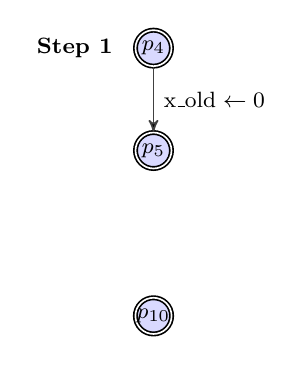
\begin{tikzpicture}[->,>=stealth',auto,node distance=2.1cm,
                    semithick,font=\footnotesize]

	\node[PRstate] (n00) {$p_4$};
	\node[PRstate] (n0) [below of=n00, yshift=0.8cm] {$p_5$};
	\node[PRstate] (n1) [below of=n0] {$p_{10}$};
	\node (label) [left of=n00, node distance=1cm] {\bf Step 1};

  \path [transition] 
		(n00) edge  node {$\lstinline|x_old| \gets 0$} (n0);
\end{tikzpicture}
\end{minipage} 
\begin{minipage}[c]{.75\textwidth}
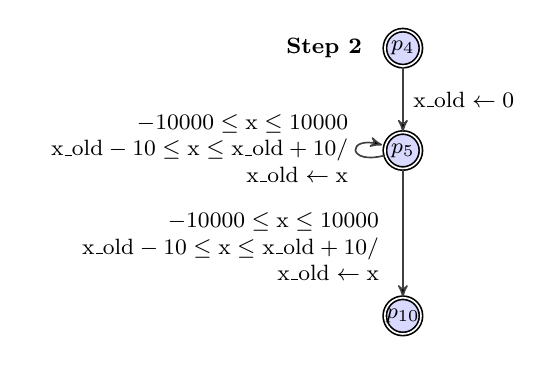
\begin{tikzpicture}[->,>=stealth',auto,node distance=2.1cm,
                    semithick,font=\footnotesize]

	\node[PRstate] (n00) {$p_4$};
	\node[PRstate] (n0) [below of=n00, yshift=0.8cm] {$p_5$};
	\node[PRstate] (n1) [below of=n0] {$p_{10}$};
	\node (label) [left of=n00, node distance=1cm] {\bf Step 2};

  \path [transition] 
		(n00) edge  node {$\lstinline|x_old| \gets 0$} (n0);
  \path [transition] 
		(n0) edge  [loop left] node [left, xshift=0.2cm] {
		$\begin{array}{r}
			-10000 \leq \lstinline|x| \leq 10000 \\
			\lstinline|x_old|-10 \leq \lstinline|x| \leq \lstinline|x_old|+10 /\\
			\lstinline|x_old| \gets \lstinline|x|
		\end{array}$
		} (n0);
  \path [transition] 
		(n0) edge node [left, yshift=-0.2cm, xshift=0] {
		$\begin{array}{r}
			-10000 \leq \lstinline|x| \leq 10000 \\
			\lstinline|x_old|-10 \leq \lstinline|x| \leq \lstinline|x_old|+10 /\\
			\lstinline|x_old| \gets \lstinline|x|
		\end{array}$
		} (n1);
\end{tikzpicture}
\end{minipage}
\caption{Ascending sequence of subgraphs}
\end{figure}


In this example, we see that our technique actually combines best of
\emph{Guided Static Analysis} and \emph{Path Focusing}. Still, we need to unroll
the loop once in order to get precise results. Section \ref{sec:disjunctive}
proposes a new technique that gives precise invariants without needing such
graph transformations.

\section{Disjunctive Invariants}
\label{sec:disjunctive}

\cite{DBLP:conf/pldi/GulwaniZ10} proposed a technique for computing disjunctive invariants, by
distinguishing all the paths inside a loop. In
this section, we propose to improve this technique by using SMT queries to find
interesting paths, the objective being to avoid an explicit exhaustive
enumeration of an exponential number of paths.

For each control point $p_i$, we compute a disjunctive invariant
$\bigvee_{1\leq j \leq m_i} X_{i,j}$. We denote by $n_i$ the number of
distinct paths starting at $p_i$.
To perform the analysis, one chooses an integer $\delta_i \in [1,m_i]$, and
a mapping function $\sigma_i: [1,m_i] \times [1,n_i] \mapsto [1,m_i]$.
  The $k$-th path starting fom $p_i$ is denoted $\tau_{i,k}$.
  The image of the $j$-th disjunct $X_{i,j}$ by the path $\tau_{i,k}$ is then
  joined with $X_{i,\sigma(j,k)}$.
Initially, the $\delta_i$-th abstract value contains the initial states of
$p_i$, and all other abstract values contain~$\emptyset$.

For each control point $p_i \in P_R$, $m_i$, $\delta_i$ and $\sigma_i$ can be defined heuristically.
For instance, one could define $\sigma_i$ so that $\sigma_i(j,k)$ only depends on the
last transition of the path, or else construct it dynamically during the
analysis.

Our method improves this technique in two ways :
\begin{compactitem}
\item Instead of enumerating the whole set of paths, we keep them implicit and
compute them only when needed.

\item At each loop iteration of the original algorithm \cite{DBLP:conf/pldi/GulwaniZ10}, an image by each path inside the loop is computed for each disjunct of the invariant candidate.
Yet, many of these images may be redundant: for instance, if our invariant candidate is $(0 \leq x \leq 10 \land 0 \leq y \leq 1000) \lor (x < -10 \land y < -10)$, then there is no point enumerating paths whose image is included in this invariant candidate.
In our approach, we compute such an image only if it makes the resulting abstract value grow.
\end{compactitem}

Our improvement consists in a modification of the SMT formula we solve in
\ref{sec:guided_multigraph}.
We introduce in this formula Boolean variables $\{d_j, 1 \leq j \leq m\}$, so
that we can easily find in the model which abstract value of the
disjunction of the source point has
to be chosen to make the invariant of the destination grow.
The resulting formula that is given to the SMT solver is defined
by $g(p_i)$.
When the formula is satisfiable, we know that the index $j$ of the starting
disjunct that has to be chosen is the one for which the associate Boolean value
$d_j$ is \emph{true} in the model. Then, we can easily compute the value of 
$\sigma_i(j,k)$, thus know the index of the disjunct to join with.
%
\vspace{-.5em}
\begin{equation*}
g(p_i) = \rho \wedge b_i^s \wedge 
\displaystyle\bigwedge_{j \in P_R \atop j \neq i} \neg b_j^s 
 \wedge 
\displaystyle\bigvee_{1 \leq k \leq m_i}\!\! (d_k \wedge X_{i,k} \wedge \bigwedge_{l \neq k}
\neg d_l)
\wedge
\displaystyle\bigvee_{j \in Succ(i)}\!\!
(b_j^d \wedge \bigwedge_{1 \leq k \leq m_i}\!\! (\neg X_{j,k}))
\vspace{-.5em}
\end{equation*}

In our algorithm, the initialization of the abstract values slightly differs from
algorithm \ref{algo:combined} line~\ref{alg=X-init}, since we now have to
initialize each disjunct. Instead of Line~\ref{alg=X-init}, we initialize $X_{i,k}$ with $\perp$ for all
$k \in \{1,..,m_i\} \setminus \{\delta_i\}$, and $X_{i,\delta_i}$ with
$\gets I_{p_i}$.

% MM: pas la place pour un vrai algo => inliné dans le texte.
% Line~\ref{alg=X-init} is then replaced by:
% %\begin{algorithm}[!h]
% \begin{algorithmic}[1] 
% \FORALL {$k \in \{1,..,m_i\} \setminus \{\delta_i\}$}
% 	\STATE $X_{i,k} \gets \perp$
% \ENDFOR
% \STATE $X_{i,\delta_i} \gets I_{p_i}$
% \end{algorithmic}
% %\end{algorithm}

Furthermore, the Path-focused algorithm (line~\ref{alg=pf} from algorithm
\ref{algo:combined}) is enhanced to deal with disjunctive invariants, and
is detailed in algorithm \ref{algo:disjunctive}.

The \emph{Update} function can classically assign  $X_{i,\sigma_i(j,k)} \widening (X_{i,\sigma_i(j,k)} \sqcup
\tau_{i,k}(X_{i,j}))$ to $X_{i,\sigma_i(j,k)}$, or can integrate the special treatment for self loops
proposed by \cite{Monniaux_Gonnord_SAS11}, with widening/narrowing sequence or
acceleration.

\vspace{-1em}
\begin{algorithm}[!h]
\caption{Disjunctive invariant computation with implicit paths}\label{gulwani2}
\label{algo:disjunctive}
\begin{algorithmic}[1] 
\WHILE {true}
	\STATE $res \gets SmtSolve\left[g(p_i)\right]$
	\IF {$res = unsat$}
		\STATE \textbf{break}
	\ENDIF
	\STATE Compute the path $\tau_{i,k}$ from $res$ 
	\STATE Take $j \in \{ l | d_l = true\}$ 
	\STATE Update($X_{i,\sigma_i(j,k)})$
\ENDWHILE
\end{algorithmic}
\end{algorithm}
\vspace{-1em}

We experimented with a heuristic
of dynamic construction of the $\sigma_i$ functions, adapted from
\cite{DBLP:conf/pldi/GulwaniZ10}. 
%\DM{Cette heuristique, je croyais que c'était nous qui l'avions trouvée,
%et qu'elle n'était pas dans Gulwani?}
%\JH{Non. Gulwani fait la même chose en un peu plus complique (voir commentaire
%suivant)}
%\MM{Du coup, la contribution~\ref{contr:disjunctive} devrait être
%  affaiblie un peu je suppose. Gulwani fait aussi du SMT-solving ?}
%\DM{Non, Gulwani énumère tous les chemins un par un à tous les coups.}
%\MM{OK, du coup j'ai ajouté une phrase à la fin de la section pour
%  rappeler notre contrib}
For each control point $p_i \in P_R$, we start with one single disjunct
($m_i = 1$) and define $\delta_i = 1$.
$M$ denotes an upper bound on the number of disjuncts per control point.

The $\sigma_i$ functions take as parameters the index of the starting abstract
value, and the path we focus on. 
Since we dynamically construct these functions
during the analysis, we store their already computed image into a
compact representation, such as Algebraic Decision Diagrams.
$\sigma_i(j,k)$ is then constructed on the fly only when needed, and computed
only once.
When the value of $\sigma_i(j,k)$ is required but undefined, we first compute
the image of the
abstract value $X_{i,j}$ by the path indexed by $k$, and try to find an existing
disjunct of index $j'$ so that the least upper bound of the two abstract values is exactly their union (using SMT-solving).
If such an index exists, then we set $\sigma_i(j,k) = j'$.
Otherwise:
\begin{compactitem}
	\item if $m_i < M$, we increase $m_i$ by $1$ and define $\sigma_i(j,k) = m_i$
	\item if $m_i = M$, we define $\sigma_i(j,k) = M$ 
		%\JH{A la place, Gulwani cherche l'invariant qui a le plus de contraintes
		%d'egalite en commun pour definir son $sigma$. Nous, on le met dans M, pour simplifier}
\end{compactitem}
The main difference with the original
algorithm~\cite{DBLP:conf/pldi/GulwaniZ10} is that we construct
$\sigma_i(j,k)$ using SMT queries instead of enumerating a possibly
exponential number of paths to find a solution.

\section{Implementation and Experimental Comparisons}
\label{sec:experiments}

We have implemented our proposed solutions inside a prototype of intraprocedural
static analyzer called PAGAI,
as well as the classical abstract interpretation algorithm, and the state-of-the-art
techniques \emph{Path Focusing} \cite{Monniaux_Gonnord_SAS11} and \emph{Guided
Static Analysis} \cite{DBLP:conf/sas/GopanR07}. It is
available online at \url{https://forge.imag.fr/projects/pagai/}. The
implementation is documented in~\cite{julien-henry-m2r}.
\MM{pas idéal de citer un rapport de M2, mais ça a des chances de
  faire taire les reviewers qui voudraient des détails sur comment
  c'est fait, et on n'a pas la place de mettre plus. Le
  paragraphe~\ref{sec:analysis-algorithm} a été supprimé depuis
  PLDI ...}

%\MM{On peut peut-être citer le nom de l'outil (on garde PAGAI ?) ici.
%  L'intérêt d'avoir un nom, c'est que les gens peuvent en parler plus
%  facilement, et c'est plus facile de retrouver le papier origine d'un
%  outil quand il cite son nom}
%\DM{Dans la version finale, oui, mais pas dans une soumission anonymisée... suffit de Googlifier pagai sur imag.fr}
%
PAGAI operates over LLVM bitcode \cite{LLVM_langref,Lattner:2004:LCF:977395.977673}, which is a target for several compilers, most notably Clang (supporting C and C++) and llvm-gcc (supporting C, C++, Fortran and Ada).
Abstract domains are provided by the APRON library \cite{DBLP:conf/cav/JeannetM09}, and include convex polyhedra (from the builtin Polka ``PK'' library), octagons, intervals, and linear congruences.
For SMT-solving, our analyzer uses Yices
\cite{DBLP:conf/cav/DutertreM06} or Microsoft Z3~\cite{DBLP:conf/tacas/MouraB08}.

We conducted extensive experiments on real-life programs in order to compare the
different techniques, mostly on open-source projects (Fig.~\ref{fig:projects}) written in C, C++ and Fortran.
\MM{TODO: résumer les conclusions sur les résultats}

\begin{figure}[h!]
      \centering
      \begin{tabular}{|l|r|r|r|r|r|r|r|} \hline
        \multicolumn{1}{|c|}{} &
        \multicolumn{2}{c|}{Size} &
        \multicolumn{5}{c|}{Execution time (seconds)} \\ \hline
        \multicolumn{1}{|c|}{Name} & 
        \multicolumn{1}{c|}{kLOC}  & 
        \multicolumn{1}{c|}{$|P_R|$}  &
        \multicolumn{1}{c|}{\textbf{S}} &
        \multicolumn{1}{c|}{\textbf{G}} &
        \multicolumn{1}{c|}{\textbf{PF}} &
        \multicolumn{1}{c|}{\textbf{G+PF}} &
	\multicolumn{1}{c|}{\textbf{DIS}} \\ 
        \hline
        % M-x align RET powers ;-).
a2ps-4.14      & 55  & 2012  & 64  & 17  & 66   & 175  & 512   \\
gawk-4.0.0     & 59  & 902   & 59  & 8   & 18   & 43   & 129   \\
gnuchess-6.0.0 & 38  & 1222  & 112 & 21  & 122  & 374  & 866   \\
gnugo-3.8      & 83  & 2801  & 155 & 31  & 128  & 382  & 1403  \\
grep-2.9       & 35  & 820   & 50  & 12  & 21   & 58   & 307   \\
gzip-1.4       & 27  & 494   & 63  & 12  & 36   & 97   & 617   \\
lapack-3.3.1   & 954 & 16422 & 721 & 246 & 2690 & 6052 & 22222 \\
make-3.82      & 34  & 993   & 22  & 7   & 32   & 83   & 255   \\
sed-4.2        & 23  & 292   & 35  & 7   & 23   & 69   & 521   \\
tar-1.26       & 73  & 1712  & 270 & 39  & 110  & 304  & 1164  \\
% TODO: mettre à jour les chiffres ?
	\hline
      \end{tabular}
      \label{fig:projects}

    % GNUPLOT: LaTeX picture with Postscript
\begingroup
  \makeatletter
  \providecommand\color[2][]{%
    \GenericError{(gnuplot) \space\space\space\@spaces}{%
      Package color not loaded in conjunction with
      terminal option `colourtext'%
    }{See the gnuplot documentation for explanation.%
    }{Either use 'blacktext' in gnuplot or load the package
      color.sty in LaTeX.}%
    \renewcommand\color[2][]{}%
  }%
  \providecommand\includegraphics[2][]{%
    \GenericError{(gnuplot) \space\space\space\@spaces}{%
      Package graphicx or graphics not loaded%
    }{See the gnuplot documentation for explanation.%
    }{The gnuplot epslatex terminal needs graphicx.sty or graphics.sty.}%
    \renewcommand\includegraphics[2][]{}%
  }%
  \providecommand\rotatebox[2]{#2}%
  \@ifundefined{ifGPcolor}{%
    \newif\ifGPcolor
    \GPcolorfalse
  }{}%
  \@ifundefined{ifGPblacktext}{%
    \newif\ifGPblacktext
    \GPblacktexttrue
  }{}%
  % define a \g@addto@macro without @ in the name:
  \let\gplgaddtomacro\g@addto@macro
  % define empty templates for all commands taking text:
  \gdef\gplbacktext{}%
  \gdef\gplfronttext{}%
  \makeatother
  \ifGPblacktext
    % no textcolor at all
    \def\colorrgb#1{}%
    \def\colorgray#1{}%
  \else
    % gray or color?
    \ifGPcolor
      \def\colorrgb#1{\color[rgb]{#1}}%
      \def\colorgray#1{\color[gray]{#1}}%
      \expandafter\def\csname LTw\endcsname{\color{white}}%
      \expandafter\def\csname LTb\endcsname{\color{black}}%
      \expandafter\def\csname LTa\endcsname{\color{black}}%
      \expandafter\def\csname LT0\endcsname{\color[rgb]{1,0,0}}%
      \expandafter\def\csname LT1\endcsname{\color[rgb]{0,1,0}}%
      \expandafter\def\csname LT2\endcsname{\color[rgb]{0,0,1}}%
      \expandafter\def\csname LT3\endcsname{\color[rgb]{1,0,1}}%
      \expandafter\def\csname LT4\endcsname{\color[rgb]{0,1,1}}%
      \expandafter\def\csname LT5\endcsname{\color[rgb]{1,1,0}}%
      \expandafter\def\csname LT6\endcsname{\color[rgb]{0,0,0}}%
      \expandafter\def\csname LT7\endcsname{\color[rgb]{1,0.3,0}}%
      \expandafter\def\csname LT8\endcsname{\color[rgb]{0.5,0.5,0.5}}%
    \else
      % gray
      \def\colorrgb#1{\color{black}}%
      \def\colorgray#1{\color[gray]{#1}}%
      \expandafter\def\csname LTw\endcsname{\color{white}}%
      \expandafter\def\csname LTb\endcsname{\color{black}}%
      \expandafter\def\csname LTa\endcsname{\color{black}}%
      \expandafter\def\csname LT0\endcsname{\color{black}}%
      \expandafter\def\csname LT1\endcsname{\color{black}}%
      \expandafter\def\csname LT2\endcsname{\color{black}}%
      \expandafter\def\csname LT3\endcsname{\color{black}}%
      \expandafter\def\csname LT4\endcsname{\color{black}}%
      \expandafter\def\csname LT5\endcsname{\color{black}}%
      \expandafter\def\csname LT6\endcsname{\color{black}}%
      \expandafter\def\csname LT7\endcsname{\color{black}}%
      \expandafter\def\csname LT8\endcsname{\color{black}}%
    \fi
  \fi
  \setlength{\unitlength}{0.0500bp}%
  \begin{picture}(5040.00,5040.00)%
    \gplgaddtomacro\gplbacktext{%
      \csname LTb\endcsname%
      \put(594,966){\makebox(0,0)[r]{\strut{} 0}}%
      \put(594,1442){\makebox(0,0)[r]{\strut{} 2}}%
      \put(594,1918){\makebox(0,0)[r]{\strut{} 4}}%
      \put(594,2394){\makebox(0,0)[r]{\strut{} 6}}%
      \put(594,2871){\makebox(0,0)[r]{\strut{} 8}}%
      \put(594,3347){\makebox(0,0)[r]{\strut{} 10}}%
      \put(594,3823){\makebox(0,0)[r]{\strut{} 12}}%
      \put(594,4299){\makebox(0,0)[r]{\strut{} 14}}%
      \put(594,4775){\makebox(0,0)[r]{\strut{} 16}}%
      \put(1216,834){\rotatebox{-45}{\makebox(0,0)[l]{\strut{}G/S}}}%
      \put(1705,834){\rotatebox{-45}{\makebox(0,0)[l]{\strut{}PF/S}}}%
      \put(2195,834){\rotatebox{-45}{\makebox(0,0)[l]{\strut{}PF/G}}}%
      \put(2685,834){\rotatebox{-45}{\makebox(0,0)[l]{\strut{}G+PF/PF}}}%
      \put(3174,834){\rotatebox{-45}{\makebox(0,0)[l]{\strut{}G+PF/G}}}%
      \put(3664,834){\rotatebox{-45}{\makebox(0,0)[l]{\strut{}G+PF/S}}}%
      \put(4153,834){\rotatebox{-45}{\makebox(0,0)[l]{\strut{}DIS/G+PF}}}%
      \put(236,2871){\rotatebox{-270}{\makebox(0,0){\strut{}percentage of control points}}}%
    }%
    \gplgaddtomacro\gplfronttext{%
      \put(3656,4602){\makebox(0,0)[r]{\strut{}$\subsetneq$}}%
      \put(3656,4382){\makebox(0,0)[r]{\strut{}$\supsetneq$}}%
      \put(3656,4162){\makebox(0,0)[r]{\strut{}uncomparable}}%
    }%
    \gplbacktext
    \put(0,0){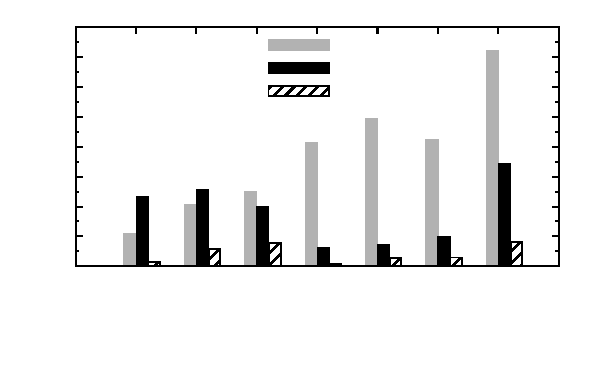
\includegraphics{gnuplot/techniques}}%
    \gplfronttext
  \end{picture}%
\endgroup

  \vspace{-20pt}
  \caption{Comparison of the abstract values obtained on several open-source projects. The table shows
  their respective number of lines of code, number of control points in $P_R$, and execution time
  on various techniques.
  Techniques are classical abstract
  interpretation (S), \emph{Guided Static
  Analysis} (G), \emph{Path-focused} technique (PF), our combined technique
  (G+PF), and its version with disjunctive invariants (DIS).
  The $\subsetneq$ bars gives the percentage of invariants stronger (more precise; smaller with respect to inclusion) with the left-side technique,
$\supsetneq$ the percentage of invariants stronger with the right-side technique,
and ``uncomparable'' gives the percentage of invariants that are uncomparable, i.e
neither greater nor smaller;
the code points where both invariants are equal make up the remaining percentage. See Tab.~\ref{tab:techniques} for details.}
  \label{fig:techniques}
\end {figure}

\MM{Bon, c'est vraiment frustrant de se limiter à ça, mais pour écrire
  plus, faut trouver de la place}
These results confirm that our combined technique improve the
analysis in comparison with the two techniques taken individually, at
a reasonable cost. The extension with disjunctive invariants increases
precision in many cases, but with higher cost in terms of execution
time.

\section{Conclusion and Future Prospects}
Roughly, an analysis by abstract interpretation is defined by the choice of an iteration strategy and an abstract domain. In this article, we demonstrated that changes in the iteration algorithm can significantly improve precision, sometimes while improving analysis times.

A common criticism of analysis techniques based on SMT-solving is that they
do not scale up. Yet, our experiments show that, for numerical properties,
they scale up to the size of typical functions and loops.
It is however
quite certain that, naively applied, they cannot scale to the kind of
programs targeted by e.g. the Astr\'ee tool, that is, a dozens or hundreds
of thousands of lines of code in a single loop operating over similar numbers
of remanent variables.
Actually, for such applications, only (quasi-)linear
algorithms scale up, and ``cheap'' abstract domains such as octagons ($O(n^3)$ where $n$ is the number of variables) are not applied to the full variable set, but to restricted subsets thereof.
It thus seems reasonable that techniques such as considering ``packs'' of related variables, slicing, etc. may similarly help SMT-based techniques to scale to global analyses.

We compared the precision of different techniques and abstract domains by comparing the invariants for the inclusion ordering. A better metric is perhaps to take a client analysis --- such as the detection of overflows and array bound violations --- and compare the rates of alarms.

We focused on numerical properties, because they are supported by easily available abstract libraries. Yet, in most programs, properties of data structures are important for proving interesting properties. Further investigations are needed not only on good abstractions for pointers (many are already known) but also on their conversion to SMT problems.

\FloatBarrier

\phantomsection\addcontentsline{toc}{section}{References} 
\bibliographystyle{splncs03}
\bibliography{implicitization}

\appendix

\MM{TODO: la partie appendix est laissée en chantier. A priori, on ne
  mettra que les tableaux de chiffres sans les commentaires, et les
  tableaux risquent de changer avec les avancées de Julien.}

\section{Experimental Results}

\subsection{Analysis Algorithm}
\label{sec:analysis-algorithm}
For each program, we distinguish a set $P_R = P_W$ of suitable widening points by a simple algorithm: for each procedure, compute the strongly connected components of its control-flow graph using Tarjan's algorithm; the targets of the back-edges of the depth-first search are added to~$P_R$. Note that the resulting set is not necessarily minimal, but is sufficient to disconnect all cycles --- more sophisticated techniques are discussed in e.g. \cite{BourdonclePhd}.

LLVM bitcode is in \emph{static single assignment} (SSA) form: a given scalar variable is given a value at a single syntactic point in the program. In concrete terms, an assignment \lstinline|x=2*x+1;| gets translated into a definition $x_2 = 2x_1+1$, with distinct variables $x_1$ and $x_2$ corresponding to the same original variable \lstinline|x| at different points in the program.
\avirer{LLVM makes it easy to follow definition-use and use-definition chains: for a given variable (say, $x_2$) one can immediately obtain its definition (say, $2x_1+1$).
One may see conversion to SSA form as a static precomputation of some of the symbolic propagations proposed by \cite{DBLP:conf/vmcai/Mine06} to enhance the precision of analyses.}

SSA introduces $\phi$-functions at the head of a control code to
define variables whose value depends on which incoming edge to this
control node was last taken. For instance, for
\lstinline|if (...) { x = 2*x+1; } else { x= 0; }|, then $x_2$ is defined as
$\phi(2x_1+1,0)$. In this framework, variables are either defined as
an arithmetic ($+$, $-$, $\times$, $/$) function of other variables,
or not be representable as affine linear functions, because they are
defined using $\phi$-functions, bitwise arithmetic, loads from memory,
or return values from function calls.

This motivates a key implement decision of our tool: only those variables $v_1,\dots,v_n$ that are not defined by arithmetic operations are retained as coordinates in the abstract domain (e.g. as dimensions in polyhedra). A basic block of code therefore amounts to a \emph{parallel assignment} operation
$(v_1,\dots,v_n) \allowbreak\mapsto\allowbreak
(f_1(v_1,\dots,v_n), \allowbreak, \dots, \allowbreak
 f_n(v_1,\dots,v_n))$;
such operations are directly supported by APRON. This has three benefits:
(i) it limits the number of dimensions in the abstract values, since polyhedra libraries typically perform worse with higher dimensions;
(ii) the abstract operation for a single path in path-focusing methods also is a (large) parallel assignment;
(iii) as suggested by \cite{DBLP:conf/vmcai/Mine06}, this approach is more precise than running abstract operations for each program line separately:
for instance, for \lstinline|y=x; z=x-y;| with precondition $x \in [0,1]$, a line-by-line interval analysis obtains $y \in [0,1]$ and $z \in [-1,1]$ while our ``en bloc'' analysis symbolically simplifies $z = x - x = 0$ and thus $z \in [0,0]$.

In the event that a node is reachable only by a single control-flow edge (which may occur because of dead code, or during the first phases of guided static analysis), the $\phi$ operation reduces to a copy of the values flowing from that edge. In this case, our tool just propagates symbolic values through the predecessor node, without introducing $\phi$-variables.

We further reduce the number of variables by projecting out those that are not live at the program point. Again, SSA use-def and def-use chains make it easy to compute liveness.

Our tool currently only operates over scalar variables from the SSA representation and thus cannot directly cope with arrays or memory accessed through pointers. We therefore run it after the ``memory to registers'' (\texttt{mem2reg}) optimization phase in LLVM, which lifts most memory accesses to scalar variables.
The remaining memory accesses are treated as undefined values, as are the return
values of function calls. For better precision, we also apply function inlining
to the program, and we unroll every loop once.

Our tool currently assumes that integer variables are unbounded mathematical integers ($\ZZ$) and floating-point variables are real (or rational) numbers. Techniques for sound analysis of bounded integers, including with wraparound, and of floating-point operations have been developed in e.g. the Astr\'ee system \cite{ASTREE_ESOP05,ASTREE_PLDI03}, but porting these techniques to our iteration schemes using SMT-solving requires supplemental work.

Our implementation of path-focusing currently does not use true acceleration techniques, as proposed by \cite{Monniaux_Gonnord_SAS11}. Instead, it simply runs widening and narrowing iterations on a single path.
The analysis is currently only forward, even though nothing in what we describe in this article is specific to forward analysis.

\subsection{Precision of the Various Techniques}
\label{sec:compare_techniques}

\MM{TODO: graphique supprimé ici}

\begin{table*}
\begin{center}
\setlength{\tabcolsep}{0.75ex}
\begin{tabular}{|l
|D{.}{.}{2}D{.}{.}{2}D{.}{.}{2}%
|D{.}{.}{2}D{.}{.}{2}D{.}{.}{2}%
|D{.}{.}{2}D{.}{.}{2}D{.}{.}{2}%
|D{.}{.}{2}D{.}{.}{2}D{.}{.}{2}%
|D{.}{.}{2}D{.}{.}{2}D{.}{.}{2}%
|D{.}{.}{2}D{.}{.}{2}D{.}{.}{2}|} \hline
\multicolumn{1}{|c|}{\textbf{Benchmark}}
& \multicolumn{3}{c|}{\textbf{G/S}}
& \multicolumn{3}{c|}{\textbf{PF/S}}
& \multicolumn{3}{c|}{\textbf{PF/G}}
& \multicolumn{3}{c|}{\textbf{G+PF/PF}}
& \multicolumn{3}{c|}{\textbf{G+PF/G}}
& \multicolumn{3}{c|}{\textbf{DIS/G+PF}} \\ %\cline{2-16}
& \multicolumn{1}{c}{$\subsetneq$} & \multicolumn{1}{c}{$\supsetneq$} & \multicolumn{1}{c|}{unc.}
& \multicolumn{1}{c}{$\subsetneq$} & \multicolumn{1}{c}{$\supsetneq$} & \multicolumn{1}{c|}{unc.}
& \multicolumn{1}{c}{$\subsetneq$} & \multicolumn{1}{c}{$\supsetneq$} & \multicolumn{1}{c|}{unc.}
& \multicolumn{1}{c}{$\subsetneq$} & \multicolumn{1}{c}{$\supsetneq$} & \multicolumn{1}{c|}{unc.}
& \multicolumn{1}{c}{$\subsetneq$} & \multicolumn{1}{c}{$\supsetneq$} & \multicolumn{1}{c|}{unc.}
& \multicolumn{1}{c}{$\subsetneq$} & \multicolumn{1}{c}{$\supsetneq$} & \multicolumn{1}{c|}{unc.} \\
 \hline
 a2ps-4.14 & .28 & 0 & 0 & 4.82 & 2.55 & 2.27 & 4.54 & 2.55 & 2.27 & 6.81 & .28 & 0 & 8.23 & 0 & 0 & 13.06 & 3.40 & .56 \\ \hline
gawk-4.0.0 & 4.62 & 0 & 0 & 3.70 & 20.37 & .92 & .92 & 22.22 & 0 & 22.22 & 0 & 0 & 11.11 & 2.77 & 0 & 16.66 & 2.77 & .92 \\ \hline
gnuchess-6.0.0 & 1.51 & 3.47 & 0 & 6.50 & 4.33 & 0 & 6.72 & 3.25 & .21 & 6.72 & 2.38 & 0 & 10.19 & 2.38 & 0 & 15.18 & 2.81 & 3.03 \\ \hline
gnugo-3.8 & .51 & 4.44 & .34 & 11.45 & 4.27 & 3.07 & 12.13 & 4.27 & 2.73 & 10.25 & 3.07 & 2.05 & 17.77 & 3.76 & .34 & 9.05 & 11.28 & 4.78 \\ \hline
grep-2.9 & 0 & 6.19 & .47 & 1.90 & 4.76 & .47 & 3.80 & 1.90 & 1.90 & 7.61 & 2.38 & 0 & 8.57 & 2.38 & 0 & 10.47 & 5.23 & .47 \\ \hline
gzip-1.4 & .58 & 7.01 & 1.75 & 1.75 & 12.86 & 1.16 & 3.50 & 8.18 & 1.16 & 15.78 & 2.92 & 1.16 & 17.54 & 1.75 & 0 & 17.54 & 15.78 & 1.16 \\ \hline
lapack-3.3.1 & 2.60 & 5.77 & .40 & 3.11 & 5.06 & 1.03 & 4.66 & 3.47 & 1.62 & 7.55 & 1.06 & 0 & 9.24 & 1.06 & .81 & 16.11 & 7.09 & 1.34 \\ \hline
make-3.82 & 2.61 & .52 & 0 & 1.82 & 6.26 & 1.82 & 1.56 & 8.09 & 1.82 & 11.74 & .52 & 0 & 6.52 & 2.34 & 1.56 & 12.27 & 4.43 & .78 \\ \hline
tar-1.26 & 4.53 & 3.27 & 0 & 5.28 & 2.77 & 0 & 2.77 & 2.01 & .75 & 7.05 & .50 & 0 & 7.05 & .25 & 0 & 9.82 & 7.05 & 1.51 \\ \hline

\end{tabular}
\end{center}
\caption{Result of the comparison of the various techniques described in this
paper: classic Abstract Interpretation (S), \emph{Guided Static Analysis} (G),
\emph{Path-focusing} (PF), our combined technique (G+PF), and its version using
disjunctive invariants (DIS). For
instance, \textbf{G/S} compares the benefits of \emph{Guided Static Analysis}
over the classic Abstract interpretation algorithm.
$\subsetneq$, $\supsetneq$ and ``unc.'' are defined as in Fig.~\ref{fig:techniques}.}
\label{tab:techniques}
\end{table*}

For each program and each pair $(T_1,T_2)$ of analysis techniques, we list
the proportion of control points in $P_R$ where $T_1$ (resp.~$T_2$) gives a
strictly stronger invariant, denoted by $\subsetneq$ (resp. $\supsetneq$),
and the proportion of control points where the invariants given by $T_1$ and
$T_2$ are uncomparable for the inclusion ordering (the remainder of the
control points are thus those for which both techniques give the same
invariant). We use convex polyhedra as the abstract domain.

Let us briefly comment the results given in more details in Table~\ref{tab:techniques} and Figure~\ref{fig:techniques}.
\emph{Guided Static Analysis} from \cite{DBLP:conf/sas/GopanR07} improves the
result of the classical Abstract Interpretation in $2.72\%$ of the control points
in $P_R$.
\emph{Path-focusing} from \cite{Monniaux_Gonnord_SAS11} gives
statistically better results, and finds better invariants than \emph{Guided
Static Analysis} in $9.89\%$ of the cases. However, it also loses precision in an
important number ($2.68\%$) of control points.
Finally, our combined technique gives the most promising results, since it is
statistically more precise than the other techniques.

The analysis using disjunctive invariants greatly improves the
precision of the analysis (for $12.06\%$ of the control points in $P_R$), at an
acceptable time cost (see Table \ref{tab:time}). \MM{TODO}

While experiencing with techniques that use SMT-solving, we encountered some
limitations due to non-linear arithmetic in the analyzed programs. Indeed, 
the SMT-solver is not able to decide the satisfiability of some SMT-formulae
expressing the semantics of non-linear programs. 
In this case, we skipped the functions for which the SMT-solver returned the
``unknown'' result.
This limitation occurred very rarely in our experiments, except for the analysis
of \emph{Lapack/Blas}, where 798 over the 1602 functions have been skipped.
\emph{Lapack/Blas} implements matrix computations, which use floating-point multiplications.

In cases where the formula is expressed in too rich a logic for the SMT-solver to deal with, a number of workarounds are possible, including:
(i) \emph{Linearization}, as per \cite{DBLP:conf/vmcai/Mine06}, which overapproximates nonlinear semantics by linear semantics.
(ii) Replacing the results of nonlinear operations by ``unknown''.
Neither is currently implemented in our tool.

Table \ref{tab:time} \MM{TODO} gives the execution time of the different analysis
techniques. It is interesting to see that \emph{Guided Static Analysis} and
\emph{Path-focusing} are sometimes faster than the classical
algorithm.
This seems due to the fact that these algorithms start on a small subset
of the graph, and then may need fewer iterations on the complete graph.
The techniques we introduce in this article are slower, but speed is still on the same order of magnitude as the older ones.

\subsection{Precision of Abstract Domains}
\label{sec:compare_domains}
\begin{table*}
\begin{center}
\setlength{\tabcolsep}{0.75ex}
\begin{tabular}{|l
|D{.}{.}{2}D{.}{.}{2}D{.}{.}{2}%
|D{.}{.}{2}D{.}{.}{2}D{.}{.}{2}%
|D{.}{.}{2}D{.}{.}{2}D{.}{.}{2}%
|D{.}{.}{2}D{.}{.}{2}D{.}{.}{2}%
|D{.}{.}{2}D{.}{.}{2}D{.}{.}{2}%
|D{.}{.}{2}D{.}{.}{2}D{.}{.}{2}|} \hline
\multicolumn{1}{|c|}{\textbf{Benchmark}}
& \multicolumn{3}{c|}{\textbf{PK/OCT}}
& \multicolumn{3}{c|}{\textbf{PK/BOX}}
& \multicolumn{3}{c|}{\textbf{OCT/BOX}}
& \multicolumn{3}{c|}{\textbf{PK/PKEQ}}
& \multicolumn{3}{c|}{\textbf{PK/GRID}}
& \multicolumn{3}{c|}{\textbf{POLY*/POLY}} \\ %\cline{2-16}
& \multicolumn{1}{c}{$\subsetneq$} & \multicolumn{1}{c}{$\supsetneq$} & \multicolumn{1}{c|}{unc.}
& \multicolumn{1}{c}{$\subsetneq$} & \multicolumn{1}{c}{$\supsetneq$} & \multicolumn{1}{c|}{unc.}
& \multicolumn{1}{c}{$\subsetneq$} & \multicolumn{1}{c}{$\supsetneq$} & \multicolumn{1}{c|}{unc.}
& \multicolumn{1}{c}{$\subsetneq$} & \multicolumn{1}{c}{$\supsetneq$} & \multicolumn{1}{c|}{unc.}
& \multicolumn{1}{c}{$\subsetneq$} & \multicolumn{1}{c}{$\supsetneq$} & \multicolumn{1}{c|}{unc.}
& \multicolumn{1}{c}{$\subsetneq$} & \multicolumn{1}{c}{$\supsetneq$} & \multicolumn{1}{c|}{unc.} \\
 \hline
 a2ps-4.14 & 4.56 & 1.39 & 0.22 & 6.86 & 1.38 & 0.44 & 6.28 & 0 & 0 & 28.75 & 0 & 0 & 23.23 & 0 & 0.60 & 3.71 & 0.22 & 0 \\ \hline
gawk-4.0.0 & 6.49 & 0 & 0 & 9.09 & 0 & 0 & 6.49 & 0 & 0 & 27.27 & 0 & 0 & 26.15 & 0 & 1.11 & 3.52 & 0 & 0 \\ \hline
gnuchess-6.0.0 & 4.27 & 2.51 & 0.33 & 6.47 & 2.50 & 0.40 & 6.52 & 1.65 & 0.08 & 36.48 & 0 & 0 & 35.74 & 0 & 0.82 & 2.88 & 1.04 & 0 \\ \hline
gnugo-3.8 & 8.26 & 1.66 & 1.15 & 11.98 & 1.03 & 1.54 & 11.53 & 0.21 & 0.21 & 34.52 & 0 & 0 & 36.46 & 0 & 0.44 & 8.93 & 1.23 & 0.29 \\ \hline
grep-2.9 & 1.60 & 1.77 & 0.88 & 4.98 & 1.06 & 1.60 & 5.69 & 0 & 0 & 27.04 & 0 & 0 & 26.86 & 0 & 0.17 & 2.86 & 0 & 0 \\ \hline
gzip-1.4 & 7.14 & 1.72 & 0.24 & 10.83 & 0.73 & 1.23 & 9.60 & 0 & 0.24 & 32.69 & 0 & 0 & 32.45 & 0 & 0.24 & 6.15 & 1.47 & 0 \\ \hline
lapack-3.3.1 & 24.96 & 1.61 & 5.13 & 54.06 & 0.57 & 5.99 & 58.42 & 0.48 & 1.02 & 64.14 & 0.06 & 0.06 & 62.50 & 0 & 1.63 & 9.55 & 0.24 & 0.01 \\ \hline
make-3.82 & 2.44 & 2.11 & 0.22 & 7.03 & 0.97 & 1.19 & 7.11 & 0.11 & 0 & 31.11 & 0 & 0 & 32.78 & 0 & 0.82 & 4.00 & 0.33 & 0.44 \\ \hline
tar-1.26 & 1.92 & 0.72 & 0.06 & 4.85 & 0.59 & 0.35 & 4.85 & 0.11 & 0 & 25.11 & 0 & 0.05 & 24.57 & 0 & 0.70 & 1.71 & 0.23 & 0.05 \\ \hline

\end{tabular}
\end{center}
\caption{Results of the comparison of the various abstract domains, when using
the same technique (G+PF). We used as abstract domains Convex Polyhedra (PK and
POLY),
Octagons (OCT), intervals (BOX), linear equalities (PKEQ) and linear congruences
(GRID). The last column compares the domain of Convex Polyhedra with the
improved widening operator from \cite{BagnaraHRZ05SCP} (POLY*), and Convex Polyhedra
using the classical widening operator (POLY). POLY and POLY* use the Parma
Polyhedral Library \cite{PPL}.
$\subsetneq$, $\supsetneq$ and ``unc.'' are defined as in Fig.~\ref{fig:techniques}.}
\label{tab:domain}
\end{table*}

For each program and each pair $(D_1,D_2)$ of abstract domains, we compare by
inclusion the invariants of the different control points in $P_R$ (where $P_R$
is defined as in \ref{sec:compare_techniques}).
The main results are given in Table \ref{tab:domain}.

Statistically, the domain of convex polyhedra gives the better results, but
commonly yields weaker invariants than the domains of octagons/intervals;
this is a known weakness of its widening operator~\cite{Monniaux_LeGuen2011}. 
The Octagon domain appears to be much better than intervals; this is
unsurprising since in most programs and libraries, bounds on loop indices are
non constant: they depend on some parameters (array sizes etc.).

The Lapack/Blas benchmarks are unusual compared to the other programs. These libraries perform matrix computations, using nested loops over indices; such programs are the prime target for polyhedral loop optimization techniques and it is therefore unsurprising that polyhedra perform very well over them.

The analysis of linear equalities (PKEQ) performs very fast compared
to other abstract domains, but yields very imprecise invariants:
it only detects relations of the form $\sum_i a_i x_i = C$ where $a_i$ and $C$ are constants.
The comparison between the domain of convex polyhedra and linear congruences
shows the percentage of points where the use of congruences refines the
invariant. This is the case for $1.04\%$ of the control points in $P_R$.

Finally, we evaluated the benefits of the improved version of the widening
operator for convex polyhedra from \cite{BagnaraHRZ05SCP}, compared to the
classical widening. We found that the improved version from
\cite{BagnaraHRZ05SCP} yields more precise invariants for $6.58\%$ of the
control points in $P_R$.

\end{document}
